\documentclass[12pt]{article}

\usepackage[utf8]{inputenc}
\usepackage{graphicx}

\title{ECSE 323 - Lab Report 1}
\author{Group 55\\Juliette Regimbal (260657238)\\Qingzhou Yang (260687570)}
\date{February 6, 2017}
\pagenumbering{gobble}
\pagenumbering{arabic}

\begin{document}
\maketitle
\setlength{\parindent}{0ex}

\section{Objective}
The objective of this lab was to begin using Quartus and ModelSim by designing circuit schematics for a 6-bit comparator (g55\_comp6) and a modulo 13 circuit (g55\_mod13), generating VHDL files for each, and then thoroughly testing them. All testing was done through simulations in software, and no circuit was ever actually deployed to the FPGA board.\\

\section{Circuit Design}
\subsection{g55\_comp6}
The first circuit designed was the 6-bit comparator. A schematic was designed as explained in the lab manual using 2 3-bit AND gates, 1 2-bit AND gate, 6 2-bit XNOR gates, 2 6-bit inputs (A and B), and a 1-bit output. The inputs A and B are the words to compare while the single bit output AeqB is a Boolean value that is true if A and B are identical.\\

\begin{figure}[h!t]
	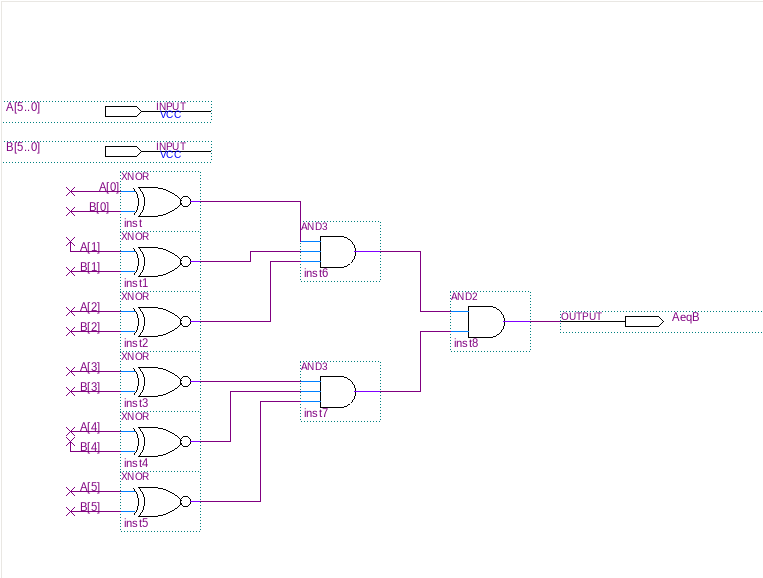
\includegraphics[scale=0.4]{graphics/comp6_schematic.png}
	\caption{\textit{g55\_comp6} Schematic}
\end{figure}

Following this the \textit{Create HDL Design File from Current File} feature was used to generate a VHDL file describing the g55\_comp6 schematic. The generated file was saved as g55\_comp6.vhd. Then another circuit was generated (g55\_lab1) that implements the g55\_comp6 as a component. The VHDL file for g55\_lab1 was too generated from a schematic.
\begin{figure}[h!t]
	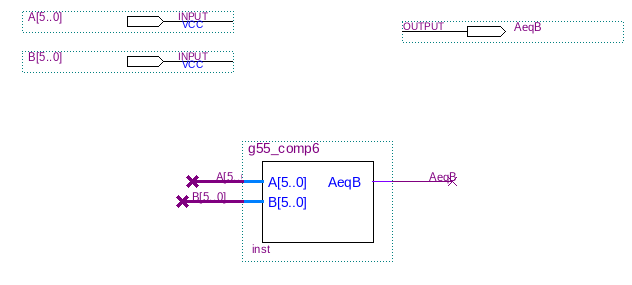
\includegraphics[scale=0.5]{graphics/lab1_schematic.png}
	\caption{\textit{g55\_lab1} Schematic}
\end{figure}

\subsection{g55\_mod13}
Following this, a circuit that computes the modulo 13 of an entered 6-bit unsigned integer was designed. As the formula for the f operation is $mod(A, B) = A -floor(A/B)*B$, multiplication and division are necessary for this circuit. To avoid the complexities associated with multiplication and division, these capabilities were implemented using addition and bit shifting, which is the equivalent of multiplying or dividing by a power of two. To streamline development, the adder was designed to be a reusable component. First a 1-bit adder with a carry-in and carry-out was designed (g55\_adder\_single) and then a second adder with two 8-bit inputs and a 9-bit output was designed building upon the g55\_adder\_single component. The 8-bit inputs were chosen to give enough room for the necessary bit shifting and the 9-bit output is including a carry-out bit.\\
\begin{figure}[h!t]
	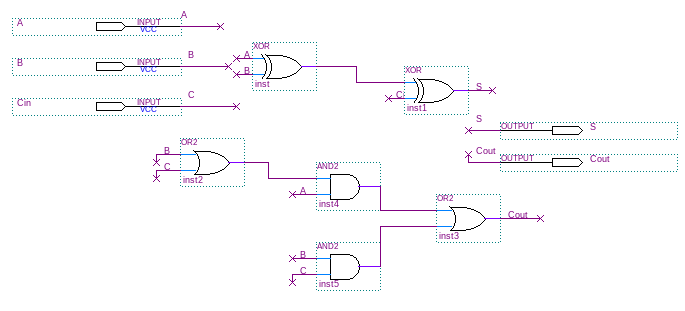
\includegraphics[scale=0.5]{graphics/adder_single_schematic.png}
	\caption{\textit{g55\_adder\_single} Schematic}
\end{figure}
\begin{figure}[h!t]
	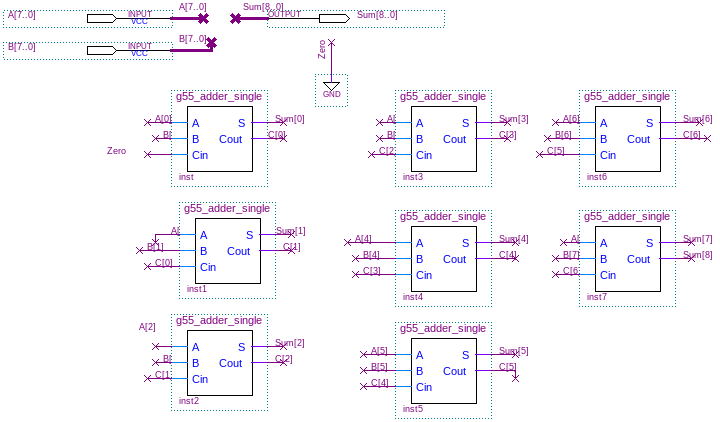
\includegraphics[scale=0.6]{graphics/adder_schematic.png}
	\caption{\textit{g55\_adder} Schematic}
\end{figure}

The modulo 13 circuit followed the operation described in the lab manual. Since in this case the modulo circuit is expressed by the equation $mod(A, 13) = A - floor(A/13)*13$ the multiplication and division by 13 must be replaced with multiplication by a power of two and addition. The division by 13 is equivalent to multiplication by 1/13 or by approximately 5/64. Since 64 is equivalent to $2^6$ it is the same as shifting right by 6 bits. 5 is equivalent to $101_2$, and $A*101_2$ can be expressed as $A_{2left} + A$ where $A_{2left}$ is A left shifted by 2 bits. If the division by 64 follows $A*5$ then there is no extra step to take the floor since any bits less than $2^0$ are lost.\\

The multiplication by 13 can be done in a similar way to multiplication by 5. 13 is $1101_2$ so $F*13 = F_{3left} + F_{2left} + F$ where $ F = floor(A*5/64)$. This only leaves the last subtraction operation. If $G = floor(A*5/64)*13$, then $A - G = A + G_{two's complement}$. The two's complement of G is found by taking the inverse and then adding 1. It is equivalent to $-G$. The result of this addition is $mod(A, 13)$. A schematic for g55\_mod13 was designed and using the same \textit{Create HDL Design File from Current File} function a VHDL file was generated. \\
\begin{figure}[h!t]
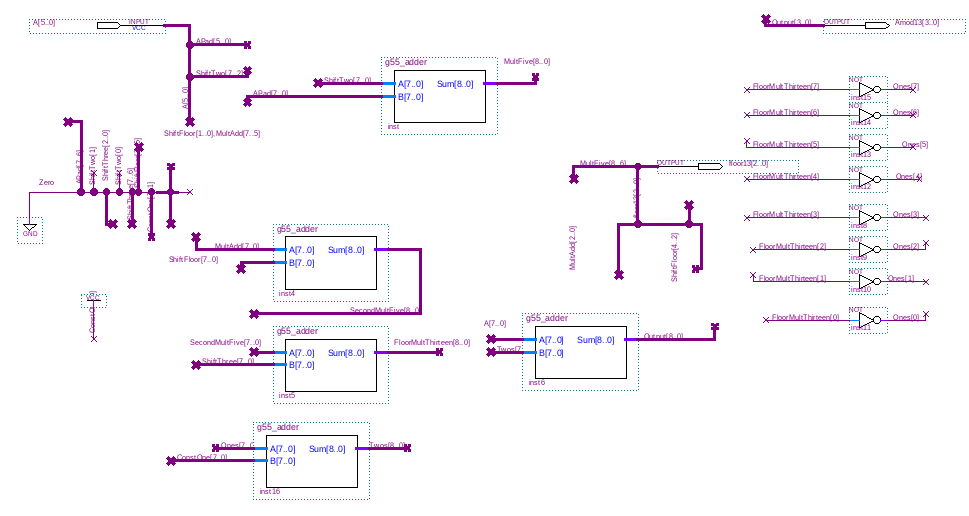
\includegraphics[scale=0.45]{graphics/mod13_schematic.png}
\caption{\textit{g55\_mod13} Schematic}
\end{figure}

\section{Testing}
\subsection{g55\_comp6}
The g55\_comp6 circuit was tested through g55\_lab1, which uses it as a component. Two testbenches were used. The first was automatically generated and only does 5 tests: when A and B are both 000000, when A is 101100 and B is 000000, when A and B are both 101100, when A is 111101 and B is 101100, and when A and B are both 111101. The output bit should be 1 in the first, third, and fifth cases and 0 in the second and fourth cases. The second test is more exhaustive, using nested for loops to check all possible combinations of A and B. The \texttt{std\_logic\_vector} and \texttt{to\_unsigned} functions are used to create words to set the inputs, and convert a loop counter to an unsigned integer word respectively.

\begin{figure}[h!t]
\centering
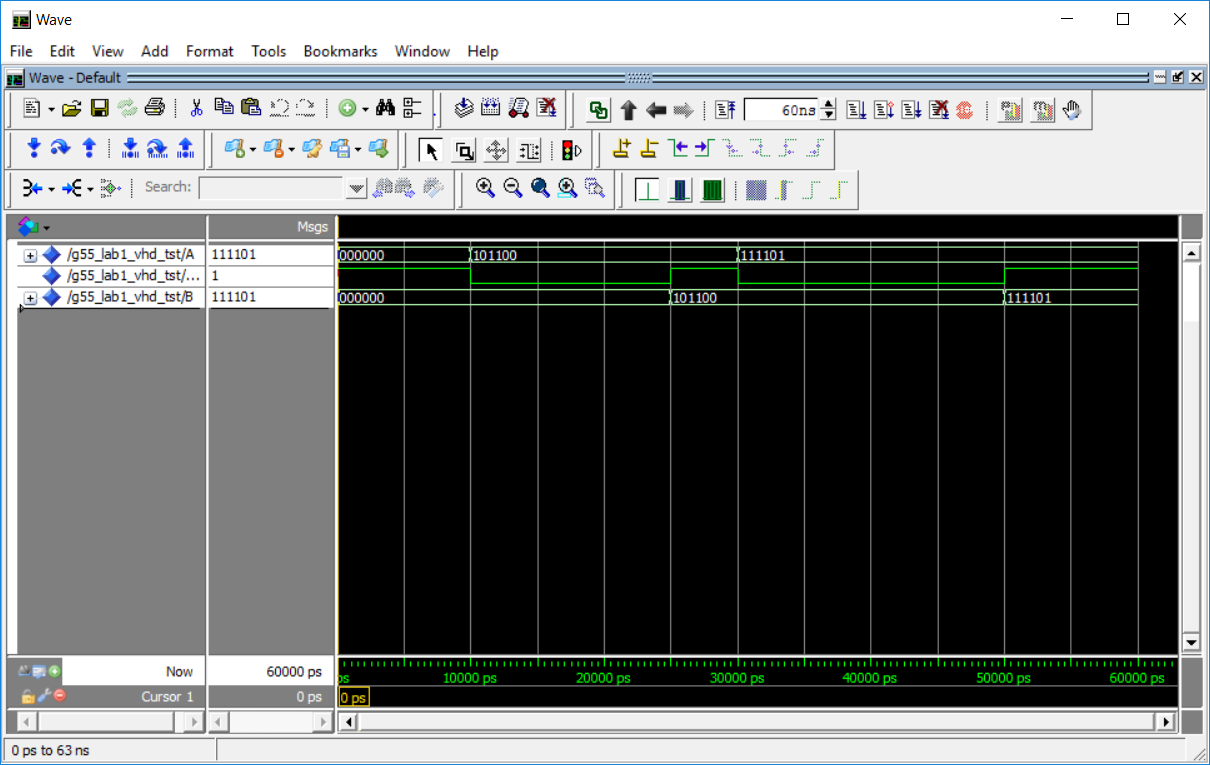
\includegraphics[scale=0.3]{graphics/comp6_wave.png}
\caption{\textit{g55\_comp6} Simple Testing}
\end{figure}
\begin{figure}[h!b]
\centering
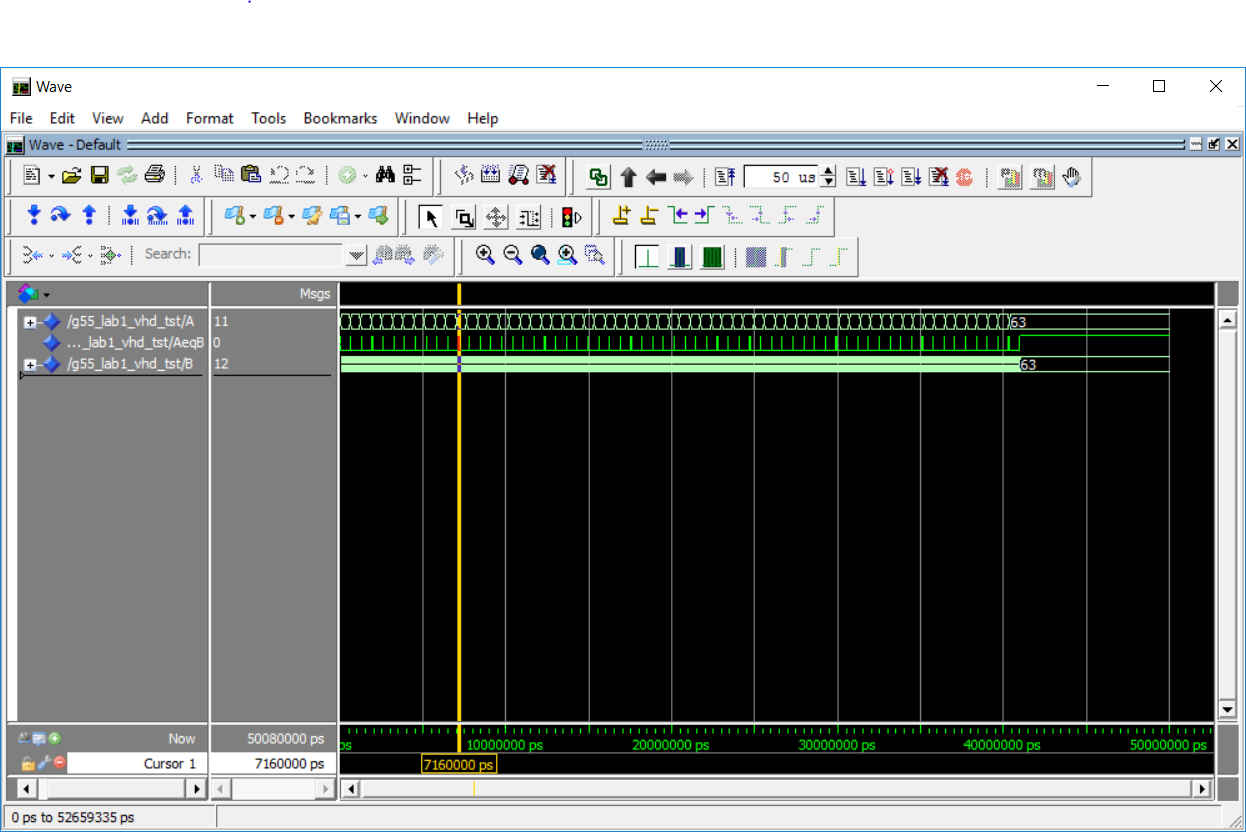
\includegraphics[scale=0.3]{graphics/comp6_wave_full.png}
\caption{\textit{g55\_comp6} Full Testing}
\end{figure}

\subsection{g55\_mod13}
Two tests were performed on the g55\_mod13 circuit and one of its components, the g55\_adder circuit. The g55\_adder is tested in a similar fashion as the g55\_comp6: all possible values of the inputs A and B are entered using nested for loops. For the sake of simplicity, the g55\_mod13 is only given 8 preset tests. It is tested with inputs 0, 3, 7, 13, 19, 27, 30 ,and 9 which should yield outputs of 0, 3, 7, 0, 6, 1, 4, and 9 respectively. The values were chosen to provide for a variety of inputs with respect to 13, including 0, an integer less than 13, equal to 13, greater than 13, and greater than 2*13.

\begin{figure}[h!t]
\centering
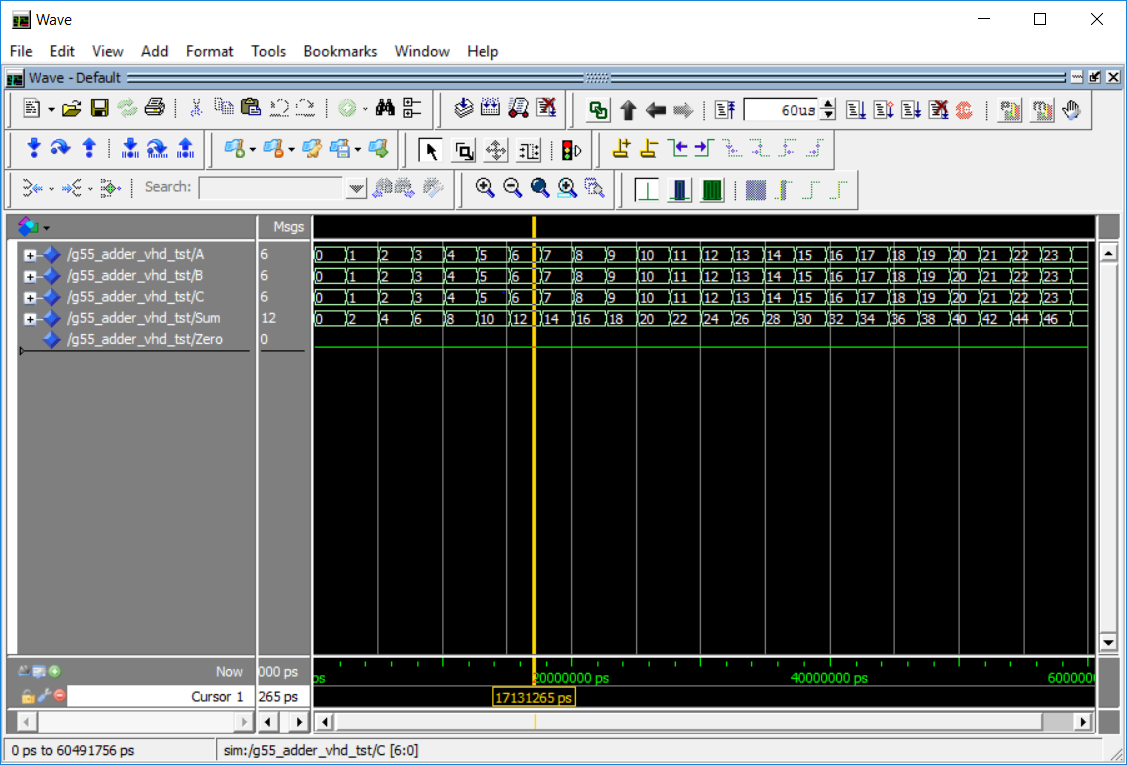
\includegraphics[scale=0.3]{graphics/adder_wave.png}
\caption{\textit{g55\_adder} Testing}
\end{figure}
\begin{figure}[h!b]
\centering
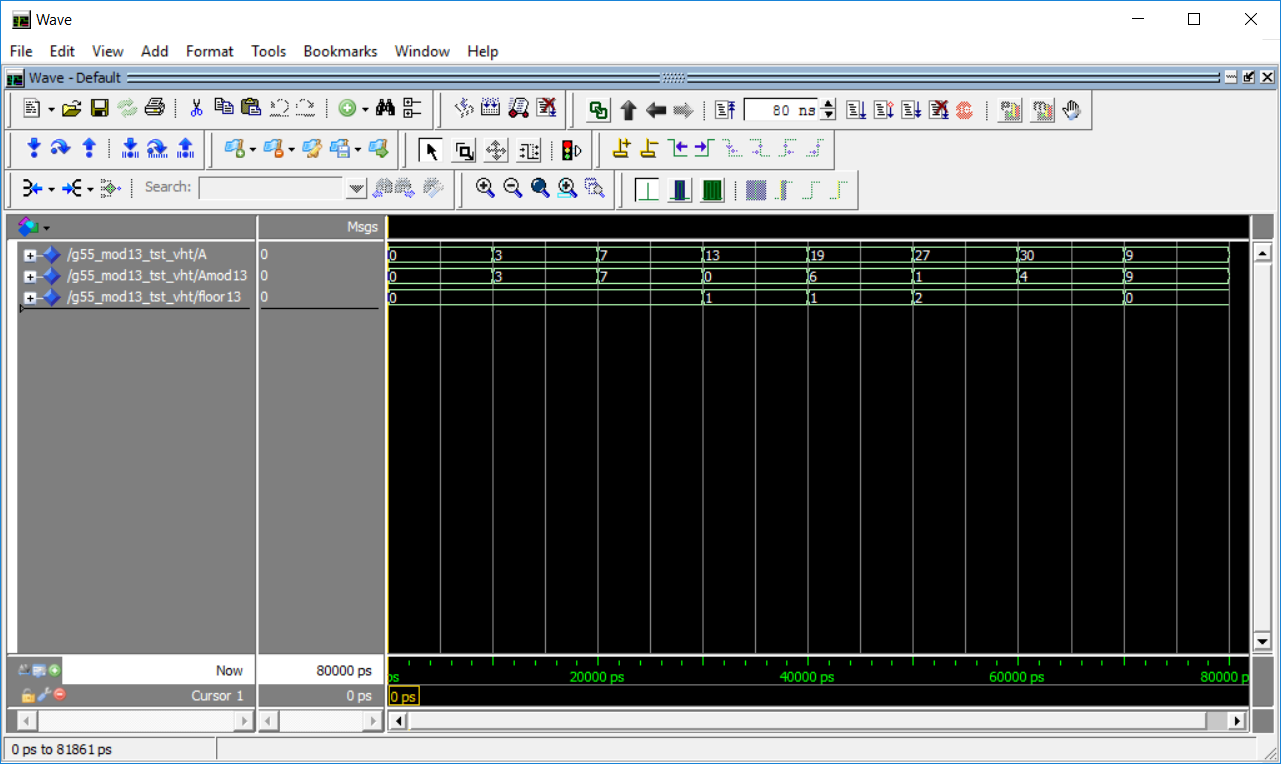
\includegraphics[scale=0.3]{graphics/mod13_wave.png}
\caption{\textit{g55\_mod13} Testing}
\end{figure}

\subsection{Results and Discussion}
All the tests ran successfully with some tweaking necessary in the case of the g55\_mod13. This success demonstrates the group's ability to design schematics for circuits, use those circuits as components in a modular way, design tests for circuits, and simulate these tests. From here more challenging designs can be attempted. Some important observations were made about the VHDL files generated from the schematics. First, in all cases the generated file is not concise. For example rather than expressing bit shifting with '\texttt{A(5 downto 3) <= B(4 downto 2);}' it would generate '\texttt{A(5) <= B(4); A(4) <= B(3); A(3) <= B(2);}'. For larger circuits this could hinder readability and make referencing old designs or debugging more difficult.\\

Also, the generated VHDL files don't always describe the schematic in the most intuitive way. What might appear to be a bus on the schematic may in fact not be, and connections between different components or signals that appear in the schematic may not be reflected properly in the VHDL. This caused some issues with debugging the g55\_mod13, with improper connections being responsible for undefined values and incorrect connections persisting in the circuit. Use of automatically generated VHDL in the future should be checked so these and similar problems do not appear.
\end{document}